\section{Introduction}\label{introduction}

\begin{frame}{Good Quote}

\large

\begin{quote}
``Simplicity is the ultimate sophistication.''

--- Leonardo da Vinci
\end{quote}

\end{frame}

\begin{frame}{Introduction}

We cover, however briefly, modeling techniques that are especially
useful to make complex relationships easier to interpret.

We will focus on:

\begin{enumerate}
\def\labelenumi{\arabic{enumi}.}
\tightlist
\item
  mediation and moderation modeling,
\item
  methods relating to structural equation modeling (SEM), and
\item
  methods applicable to our field from machine learning.
\end{enumerate}

\end{frame}

\begin{frame}{Introduction}

\begin{block}{An Aside}

Although machine learning may appear very different than mediation and
SEM, they each have advantages that can help in different situations.

\begin{itemize}
\tightlist
\item
  For example, SEM is useful when we know there is a high degree of
  measurement error or our data has multiple indicators for each
  construct.
\item
  On the other hand, regularized regression and random forests--two
  popular forms of machine learning--are great to explore patterns and
  relationships there are hundreds or thousands of variables that may
  predict an outcome.
\end{itemize}

\end{block}

\end{frame}

\section{Mediation Modeling}\label{mediation-modeling}

\begin{frame}[fragile]{Mediation Modeling}

Mediation modeling can be done via several packages.

SEM framework: + \texttt{lavaan} (stands for ``latent variable
analysis'')\footnote<.->{The \texttt{lavaan} package has some great
  vignettes at \url{http://lavaan.ugent.be/} to help with the other
  types of models it can handle.}. Although it is technically still a
``beta'' version, it performs very well especially for more simple
models.

Other good ones: + \texttt{mediation} + \texttt{RMediation}

\end{frame}

\begin{frame}{Mediation Modeling}

We model the following mediation model: \[
depression = \beta_0 + \beta_1 asthma + \epsilon_1
\]

\[
time_{Sedentary} = \lambda_0 + \lambda_1 asthma + \lambda_2 depression + \epsilon_2
\]

In essence, we believe that asthma increases depression which in turn
increases the amount of time spent being sedentary.

\end{frame}

\begin{frame}[fragile]{Mediation Modeling}

\footnotesize

\begin{Shaded}
\begin{Highlighting}[]
\KeywordTok{library}\NormalTok{(lavaan)}
\NormalTok{df}\OperatorTok{$}\NormalTok{sed_hr =}\StringTok{ }\NormalTok{df}\OperatorTok{$}\NormalTok{sed}\OperatorTok{/}\DecValTok{60}\NormalTok{  ## in hours instead of minutes}

\NormalTok{## Our model}
\NormalTok{model1 <-}\StringTok{ '}
\StringTok{  dep ~ asthma}
\StringTok{  sed_hr ~ dep + asthma}
\StringTok{'}
\NormalTok{## sem function to run the model}
\NormalTok{fit <-}\StringTok{ }\KeywordTok{sem}\NormalTok{(model1, }\DataTypeTok{data =}\NormalTok{ df)}
\KeywordTok{summary}\NormalTok{(fit)}
\end{Highlighting}
\end{Shaded}

\end{frame}

\begin{frame}[fragile]{Mediation Modeling}

\tiny

\begin{verbatim}
## lavaan (0.5-23.1097) converged normally after  30 iterations
## 
##                                                   Used       Total
##   Number of observations                          4614        4632
## 
##   Estimator                                         ML
##   Minimum Function Test Statistic                0.000
##   Degrees of freedom                                 0
## 
## Parameter Estimates:
## 
##   Information                                 Expected
##   Standard Errors                             Standard
## 
## Regressions:
##                    Estimate  Std.Err  z-value  P(>|z|)
##   dep ~                                               
##     asthma            1.478    0.183    8.084    0.000
##   sed_hr ~                                            
##     dep               0.044    0.011    3.929    0.000
##     asthma            0.412    0.139    2.965    0.003
## 
## Variances:
##                    Estimate  Std.Err  z-value  P(>|z|)
##    .dep              19.597    0.408   48.031    0.000
##    .sed_hr           11.171    0.233   48.031    0.000
\end{verbatim}

\end{frame}

\begin{frame}{Mediation Modeling}

From the output we see asthma does predict depression and depression
does predict time being sedentary. There is also a direct effect of
asthma on sedentary behavior even after controlling for depression. We
can further specify the model to have it give us the indirect effect and
direct effects tested.

\end{frame}

\begin{frame}[fragile]{Mediation Modeling}

\footnotesize

\begin{Shaded}
\begin{Highlighting}[]
\NormalTok{## Our model}
\NormalTok{model2 <-}\StringTok{ '}
\StringTok{  dep ~ a*asthma}
\StringTok{  sed_hr ~ b*dep + c*asthma}
\StringTok{ }
\StringTok{  indirect := a*b}
\StringTok{  total := c + a*b}
\StringTok{'}
\NormalTok{## sem function to run the model}
\NormalTok{fit2 <-}\StringTok{ }\KeywordTok{sem}\NormalTok{(model2, }\DataTypeTok{data =}\NormalTok{ df)}
\KeywordTok{summary}\NormalTok{(fit2)}
\end{Highlighting}
\end{Shaded}

\end{frame}

\begin{frame}[fragile]{Mediation Modeling}

\tiny

\begin{verbatim}
## lavaan (0.5-23.1097) converged normally after  30 iterations
## 
##                                                   Used       Total
##   Number of observations                          4614        4632
## 
##   Estimator                                         ML
##   Minimum Function Test Statistic                0.000
##   Degrees of freedom                                 0
## 
## Parameter Estimates:
## 
##   Information                                 Expected
##   Standard Errors                             Standard
## 
## Regressions:
##                    Estimate  Std.Err  z-value  P(>|z|)
##   dep ~                                               
##     asthma     (a)    1.478    0.183    8.084    0.000
##   sed_hr ~                                            
##     dep        (b)    0.044    0.011    3.929    0.000
##     asthma     (c)    0.412    0.139    2.965    0.003
## 
## Variances:
##                    Estimate  Std.Err  z-value  P(>|z|)
##    .dep              19.597    0.408   48.031    0.000
##    .sed_hr           11.171    0.233   48.031    0.000
## 
## Defined Parameters:
##                    Estimate  Std.Err  z-value  P(>|z|)
##     indirect          0.065    0.018    3.534    0.000
##     total             0.477    0.138    3.448    0.001
\end{verbatim}

\end{frame}

\begin{frame}[fragile]{Mediation Modeling}

We defined a few things in the model.

\begin{enumerate}
\def\labelenumi{\arabic{enumi}.}
\tightlist
\item
  We gave the coefficients labels of \texttt{a}, \texttt{b}, and
  \texttt{c}.
\item
  Doing so allows us to define the \texttt{indirect} and \texttt{total}
  effects. Here we see the indirect effect, although small, is
  significant at \(p < .001\). The total effect is larger (not
  surprising) and is also significant.
\end{enumerate}

Also note that we can make the regression equations have other
covariates as well if we needed to (i.e.~control for age or gender) just
as we do in regular regression.

\end{frame}

\begin{frame}[fragile]{Mediation Modeling}

\footnotesize

\begin{Shaded}
\begin{Highlighting}[]
\NormalTok{## Our model}
\NormalTok{model2.}\DecValTok{1}\NormalTok{ <-}\StringTok{ '}
\StringTok{  dep ~ asthma + ridageyr}
\StringTok{  sed_hr ~ dep + asthma + ridageyr}
\StringTok{'}
\NormalTok{## sem function to run the model}
\NormalTok{fit2.}\DecValTok{1}\NormalTok{ <-}\StringTok{ }\KeywordTok{sem}\NormalTok{(model2.}\DecValTok{1}\NormalTok{, }\DataTypeTok{data =}\NormalTok{ df)}
\KeywordTok{summary}\NormalTok{(fit2.}\DecValTok{1}\NormalTok{)}
\end{Highlighting}
\end{Shaded}

\end{frame}

\begin{frame}[fragile]{Mediation Modeling}

\tiny

\begin{verbatim}
## lavaan (0.5-23.1097) converged normally after  33 iterations
## 
##                                                   Used       Total
##   Number of observations                          4614        4632
## 
##   Estimator                                         ML
##   Minimum Function Test Statistic                0.000
##   Degrees of freedom                                 0
##   Minimum Function Value               0.0000000000000
## 
## Parameter Estimates:
## 
##   Information                                 Expected
##   Standard Errors                             Standard
## 
## Regressions:
##                    Estimate  Std.Err  z-value  P(>|z|)
##   dep ~                                               
##     asthma            1.462    0.183    7.980    0.000
##     ridageyr         -0.005    0.004   -1.330    0.183
##   sed_hr ~                                            
##     dep               0.044    0.011    3.927    0.000
##     asthma            0.412    0.139    2.956    0.003
##     ridageyr         -0.000    0.003   -0.063    0.950
## 
## Variances:
##                    Estimate  Std.Err  z-value  P(>|z|)
##    .dep              19.590    0.408   48.031    0.000
##    .sed_hr           11.171    0.233   48.031    0.000
\end{verbatim}

\end{frame}

\begin{frame}[fragile]{Mediation Modeling}

Although we don't show it here, we can also do moderation
(``interactions'') as part of the mediation model.

This is best done through packages other than \texttt{lavaan}.

\end{frame}

\section{Structural Equation
Modeling}\label{structural-equation-modeling}

\begin{frame}[fragile]{Structural Equation Modeling}

Instead of summing our depression variable, we can use SEM to run the
mediation model from above but use the latent variable of depression
instead. \footnotesize

\begin{Shaded}
\begin{Highlighting}[]
\NormalTok{## Our model}
\NormalTok{model3 <-}\StringTok{ '}
\StringTok{  dep1 =~ dpq010 + dpq020 + dpq030 + dpq040 + dpq050 + dpq060 + dpq070 + dpq080 + dpq090}
\StringTok{  dep1 ~ a*asthma}
\StringTok{  sed_hr ~ b*dep1 + c*asthma}

\StringTok{  indirect := a*b}
\StringTok{  total := c + a*b}
\StringTok{'}
\NormalTok{## sem function to run the model}
\NormalTok{fit3 <-}\StringTok{ }\KeywordTok{sem}\NormalTok{(model3, }\DataTypeTok{data =}\NormalTok{ df)}
\KeywordTok{summary}\NormalTok{(fit3)}
\end{Highlighting}
\end{Shaded}

\end{frame}

\begin{frame}[fragile]{Structural Equation Modeling}

\tiny

\begin{verbatim}
## lavaan (0.5-23.1097) converged normally after  47 iterations
## 
##                                                   Used       Total
##   Number of observations                          4614        4632
## 
##   Estimator                                         ML
##   Minimum Function Test Statistic             1065.848
##   Degrees of freedom                                43
##   P-value (Chi-square)                           0.000
## 
## Parameter Estimates:
## 
##   Information                                 Expected
##   Standard Errors                             Standard
## 
## Latent Variables:
##                    Estimate  Std.Err  z-value  P(>|z|)
##   dep1 =~                                             
##     dpq010            1.000                           
##     dpq020            1.096    0.024   45.136    0.000
##     dpq030            1.133    0.031   36.908    0.000
##     dpq040            1.149    0.030   38.066    0.000
##     dpq050            0.933    0.025   36.773    0.000
##     dpq060            0.929    0.022   42.107    0.000
##     dpq070            0.871    0.022   39.760    0.000
##     dpq080            0.686    0.019   36.325    0.000
##     dpq090            0.308    0.011   28.544    0.000
## 
## Regressions:
##                    Estimate  Std.Err  z-value  P(>|z|)
##   dep1 ~                                              
##     asthma     (a)    0.173    0.023    7.656    0.000
##   sed_hr ~                                            
##     dep1       (b)    0.342    0.105    3.275    0.001
##     asthma     (c)    0.418    0.139    2.998    0.003
## 
## Variances:
##                    Estimate  Std.Err  z-value  P(>|z|)
##    .dpq010            0.306    0.007   42.008    0.000
##    .dpq020            0.212    0.006   37.549    0.000
##    .dpq030            0.559    0.013   43.807    0.000
##    .dpq040            0.514    0.012   43.302    0.000
##    .dpq050            0.384    0.009   43.862    0.000
##    .dpq060            0.221    0.005   40.808    0.000
##    .dpq070            0.249    0.006   42.420    0.000
##    .dpq080            0.217    0.005   44.038    0.000
##    .dpq090            0.090    0.002   46.106    0.000
##    .sed_hr           11.179    0.233   48.012    0.000
##    .dep1              0.256    0.010   24.657    0.000
## 
## Defined Parameters:
##                    Estimate  Std.Err  z-value  P(>|z|)
##     indirect          0.059    0.020    3.019    0.003
##     total             0.477    0.138    3.448    0.001
\end{verbatim}

\end{frame}

\begin{frame}[fragile]{Structural Equation Modeling}

We defined \texttt{dep1} as a latent variable using
\texttt{=\textasciitilde{}}.

\begin{block}{Model Fit}

Although the model does not fit the data
well--``\texttt{P-value\ (Chi-square)\ =\ 0.000}''--it is informative
for demonstration. We would likely need to find out how the measurement
model
(\texttt{dep1\ =\textasciitilde{}\ dpq010\ +\ dpq020\ +\ dpq030\ +})
actually fits before throwing it into a mediation model. We can do that
via:

\end{block}

\end{frame}

\begin{frame}[fragile]{Structural Equation Modeling}

\scriptsize

\begin{Shaded}
\begin{Highlighting}[]
\NormalTok{model4 <-}\StringTok{ '}
\StringTok{  dep1 =~ dpq010 + dpq020 + dpq030 + dpq040 + dpq050 + dpq060 + dpq070 + dpq080 + dpq090}
\StringTok{'}
\NormalTok{fit4 <-}\StringTok{ }\KeywordTok{cfa}\NormalTok{(model4, }\DataTypeTok{data=}\NormalTok{df)}
\KeywordTok{summary}\NormalTok{(fit4)}
\end{Highlighting}
\end{Shaded}

\end{frame}

\begin{frame}[fragile]{Structural Equation Modeling}

\tiny

\begin{verbatim}
## lavaan (0.5-23.1097) converged normally after  29 iterations
## 
##   Number of observations                          4632
## 
##   Estimator                                         ML
##   Minimum Function Test Statistic              985.831
##   Degrees of freedom                                27
##   P-value (Chi-square)                           0.000
## 
## Parameter Estimates:
## 
##   Information                                 Expected
##   Standard Errors                             Standard
## 
## Latent Variables:
##                    Estimate  Std.Err  z-value  P(>|z|)
##   dep1 =~                                             
##     dpq010            1.000                           
##     dpq020            1.097    0.024   45.383    0.000
##     dpq030            1.128    0.031   36.962    0.000
##     dpq040            1.145    0.030   38.136    0.000
##     dpq050            0.927    0.025   36.630    0.000
##     dpq060            0.930    0.022   42.294    0.000
##     dpq070            0.870    0.022   39.941    0.000
##     dpq080            0.681    0.019   36.350    0.000
##     dpq090            0.307    0.011   28.609    0.000
## 
## Variances:
##                    Estimate  Std.Err  z-value  P(>|z|)
##    .dpq010            0.306    0.007   42.051    0.000
##    .dpq020            0.211    0.006   37.470    0.000
##    .dpq030            0.560    0.013   43.909    0.000
##    .dpq040            0.515    0.012   43.400    0.000
##    .dpq050            0.390    0.009   44.041    0.000
##    .dpq060            0.221    0.005   40.835    0.000
##    .dpq070            0.249    0.006   42.461    0.000
##    .dpq080            0.216    0.005   44.149    0.000
##    .dpq090            0.090    0.002   46.195    0.000
##     dep1              0.261    0.011   24.765    0.000
\end{verbatim}

\end{frame}

\begin{frame}[fragile]{Structural Equation Modeling}

Lack of fit in the measurement model.

\begin{itemize}
\tightlist
\item
  It is possible that these depression questions could be measuring more
  than one factor.
\item
  We could explore this using exploratory factor analysis.
\item
  We don't demonstrate that here, but know that it is possible to do in
  \texttt{R} with a few other packages.
\end{itemize}

\end{frame}

\section{Machine Learning Techniques}\label{machine-learning-techniques}

\begin{frame}{Machine Learning Techniques}

We are briefly going to introduce some machine learning techniques that
may be of interest to researchers. We will quickly introduce and
demonstrate:

\begin{enumerate}
\def\labelenumi{\arabic{enumi}.}
\tightlist
\item
  Ridge, Lasso and Elastic Net
\item
  Random Forests
\end{enumerate}

\end{frame}

\begin{frame}[fragile]{Ridge, Lasso and Elastic Net}

Use the fantastic \texttt{glmnet} package.

\begin{itemize}
\tightlist
\item
  Using the \texttt{cv.glmnet()} function we can run the ridge
  (\(alpha = 0\)), lasso (\(alpha = 1\) which is default), and elastic
  net (\(0 \leq alpha \leq 1\)).
\item
  It turns out that elastic net is the combination of the ridge and
  lasso methods and the closer \texttt{alpha} is to 1 the more it acts
  like lasso and the closer it is to 0 the more it acts like ridge.
\end{itemize}

\end{frame}

\begin{frame}{Ridge, Lasso and Elastic Net}

\begin{block}{Lasso and Elastic Net}

\begin{itemize}
\tightlist
\item
  variable selection
\item
  large number of predictors
\item
  good prediction
\end{itemize}

\end{block}

\begin{block}{Ridge}

\begin{itemize}
\tightlist
\item
  handles multi-collinearity
\item
  large number of predictors
\item
  good prediction
\end{itemize}

To learn more see ``Introduction to Statistical Learning'' by Daniela
Witten, Gareth James, Robert Tibshirani, and Trevor Hastie. A free PDF
is available on their website.

\end{block}

\end{frame}

\begin{frame}[fragile]{glmnet}

To use the package, it wants the data in a very specific form.

\begin{enumerate}
\def\labelenumi{\arabic{enumi}.}
\tightlist
\item
  We need to remove any missingness. We use \texttt{na.omit()} to do
  this.
\item
  We take all the predictors (without the outcome) and put it in a data
  matrix object. We only include a few for the demonstration but you can
  include \emph{many} predictors. We name ours \texttt{X}.
\item
  \texttt{Y} (a vector) is our outcome.
\end{enumerate}

\end{frame}

\begin{frame}[fragile]{Ridge, Lasso and Elastic Net}

\begin{block}{Prep the Data}

\begin{Shaded}
\begin{Highlighting}[]
\NormalTok{df2 <-}\StringTok{ }\NormalTok{df }\OperatorTok
\StringTok{  }\NormalTok{dplyr}\OperatorTok{::}\KeywordTok{select}\NormalTok{(riagendr, ridageyr, ridreth3, race, famsize, dep, asthma, sed_hr) }\OperatorTok
\StringTok{  }\NormalTok{na.omit}
\NormalTok{X <-}\StringTok{ }\NormalTok{df2 }\OperatorTok
\StringTok{  }\NormalTok{dplyr}\OperatorTok{::}\KeywordTok{select}\NormalTok{(}\OperatorTok{-}\NormalTok{sed_hr) }\OperatorTok
\StringTok{  }\NormalTok{data.matrix}
\NormalTok{Y <-}\StringTok{ }\NormalTok{df2}\OperatorTok{$}\NormalTok{sed_hr}
\end{Highlighting}
\end{Shaded}

\end{block}

\end{frame}

\begin{frame}[fragile]{Ridge, Lasso and Elastic Net}

Use the \texttt{cv.glmnet()} function to fit the different models.

\begin{itemize}
\tightlist
\item
  The ``cv'' refers to cross-validation\footnote<.->{Cross-validation is
    a common way to reduce over-fitting and make sure your model is
    generalizable. Generally, you split your data into training and
    testing sets. We recommend using it as often as you can, especially
    with these methods but also to make sure your other models are
    accurate on new data as well.}, which we don't discuss here, but it
  an important topic to become familiar with. Below we fit a ridge, a
  lasso, and an elastic net model.
\item
  The elastic net model uses more of the lasso penalty because the
  \texttt{alpha} is closer to 1 than 0.
\end{itemize}

\begin{Shaded}
\begin{Highlighting}[]
\KeywordTok{library}\NormalTok{(glmnet)}

\NormalTok{fit_ridge <-}\StringTok{ }\KeywordTok{cv.glmnet}\NormalTok{(X, Y, }\DataTypeTok{alpha =} \DecValTok{0}\NormalTok{)}
\NormalTok{fit_lasso <-}\StringTok{ }\KeywordTok{cv.glmnet}\NormalTok{(X, Y, }\DataTypeTok{alpha =} \DecValTok{1}\NormalTok{)}
\NormalTok{fit_enet  <-}\StringTok{ }\KeywordTok{cv.glmnet}\NormalTok{(X, Y, }\DataTypeTok{alpha =}\NormalTok{ .}\DecValTok{8}\NormalTok{)}
\end{Highlighting}
\end{Shaded}

\end{frame}

\begin{frame}[fragile]{Ridge, Lasso and Elastic Net}

Selecting an appropriate tuning parameter is best done with plots.

\begin{itemize}
\tightlist
\item
  These plots show where appropriate \texttt{lambda} values are based on
  the mean squared error of the cross-validated prediction.
\item
  The vertical dashed lines show a reasonable range of lambda values
  that can be used.
\end{itemize}

\end{frame}

\begin{frame}[fragile]{Ridge, Lasso and Elastic Net}

\begin{block}{For example}

\begin{Shaded}
\begin{Highlighting}[]
\KeywordTok{plot}\NormalTok{(fit_enet)}
\end{Highlighting}
\end{Shaded}

\end{block}

\end{frame}

\begin{frame}{Ridge, Lasso and Elastic Net}

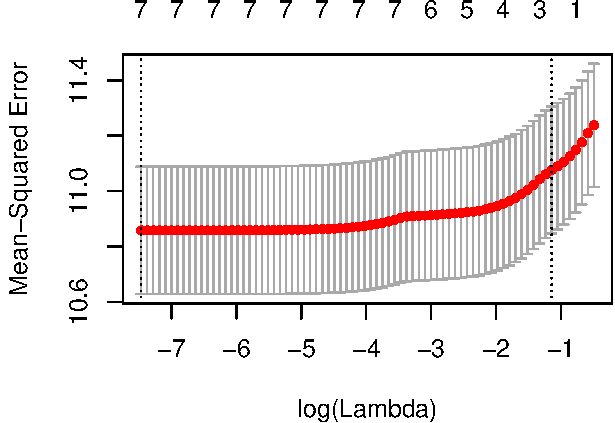
\includegraphics{07_OtherModels_files/figure-beamer/unnamed-chunk-15-1.pdf}

\end{frame}

\begin{frame}[fragile]{Ridge, Lasso and Elastic Net}

We can get the coefficients at a reasonable \texttt{lambda}.

\begin{itemize}
\tightlist
\item
  Specifically, we use the ``1-SE rule'' (near the right hand side
  vertical dashed lines in the above plots) by
  \texttt{s\ =\ "lambda.1se"}.
\item
  You can directly tell it what \texttt{lambda} value you'd like but
  this is a simple rule of thumb.
\end{itemize}

\begin{Shaded}
\begin{Highlighting}[]
\KeywordTok{coef}\NormalTok{(fit_ridge, }\DataTypeTok{s =} \StringTok{"lambda.1se"}\NormalTok{)}
\KeywordTok{coef}\NormalTok{(fit_lasso, }\DataTypeTok{s =} \StringTok{"lambda.1se"}\NormalTok{)}
\KeywordTok{coef}\NormalTok{(fit_enet, }\DataTypeTok{s =} \StringTok{"lambda.1se"}\NormalTok{)}
\end{Highlighting}
\end{Shaded}

\end{frame}

\begin{frame}[fragile]{Ridge, Lasso and Elastic Net}

\tiny

\begin{verbatim}
## 8 x 1 sparse Matrix of class "dgCMatrix"
##                         1
## (Intercept)  6.039337e+00
## riagendr     8.351244e-03
## ridageyr    -9.484185e-05
## ridreth3     1.145168e-02
## race         1.777208e-02
## famsize     -7.278221e-03
## dep          1.890571e-03
## asthma       1.891846e-02
\end{verbatim}

\begin{verbatim}
## 8 x 1 sparse Matrix of class "dgCMatrix"
##                     1
## (Intercept) 5.7065357
## riagendr    .        
## ridageyr    .        
## ridreth3    .        
## race        0.1354815
## famsize     .        
## dep         .        
## asthma      .
\end{verbatim}

\begin{verbatim}
## 8 x 1 sparse Matrix of class "dgCMatrix"
##                     1
## (Intercept) 5.4775407
## riagendr    .        
## ridageyr    .        
## ridreth3    .        
## race        0.2047703
## famsize     .        
## dep         .        
## asthma      .
\end{verbatim}

\end{frame}

\begin{frame}{Ridge, Lasso and Elastic Net}

Although we briefly introduce these regression methods, they are indeed
very important. We highly recommend learning more about them.

\end{frame}

\begin{frame}{Random Forests}

Random forests is another machine learning method that can do fantastic
prediction.

It is built in a very different way than the methods we have discussed
up to this point. It is not built on a linear modeling scheme; rather,
it is built on classification and regression trees (CART).

Again, ``Introduction to Statistical Learning'' is a great resource to
learn more.

\end{frame}

\begin{frame}[fragile]{Random Forests}

Use the \texttt{randomForest} package.

\begin{itemize}
\tightlist
\item
  We specify the model by the formula
  \texttt{sed\_hr\ \textasciitilde{}\ .} which means we want
  \texttt{sed\_hr} to be the outcome and all the rest of the variables
  to be predictors.
\end{itemize}

\begin{Shaded}
\begin{Highlighting}[]
\KeywordTok{library}\NormalTok{(randomForest)}

\NormalTok{fit_rf <-}\StringTok{ }\KeywordTok{randomForest}\NormalTok{(sed_hr }\OperatorTok{~}\StringTok{ }\NormalTok{., }\DataTypeTok{data =}\NormalTok{ df2)}
\NormalTok{fit_rf}
\end{Highlighting}
\end{Shaded}

\end{frame}

\begin{frame}[fragile]{Random Forests}

\tiny

\begin{verbatim}
## randomForest 4.6-12
\end{verbatim}

\begin{verbatim}
## Type rfNews() to see new features/changes/bug fixes.
\end{verbatim}

\begin{verbatim}
## 
## Attaching package: 'randomForest'
\end{verbatim}

\begin{verbatim}
## The following object is masked from 'package:dplyr':
## 
##     combine
\end{verbatim}

\begin{verbatim}
## The following object is masked from 'package:ggplot2':
## 
##     margin
\end{verbatim}

\begin{verbatim}
## 
## Call:
##  randomForest(formula = sed_hr ~ ., data = df2) 
##                Type of random forest: regression
##                      Number of trees: 500
## No. of variables tried at each split: 2
## 
##           Mean of squared residuals: 10.82932
##                     % Var explained: 3.64
\end{verbatim}

\end{frame}

\begin{frame}[fragile]{Random Forests}

We can find out which variables were important in the model via:

\begin{Shaded}
\begin{Highlighting}[]
\KeywordTok{par}\NormalTok{(}\DataTypeTok{mfrow=}\KeywordTok{c}\NormalTok{(}\DecValTok{1}\NormalTok{,}\DecValTok{1}\NormalTok{))  ## back to one plot per page}
\KeywordTok{varImpPlot}\NormalTok{(fit_rf)}
\end{Highlighting}
\end{Shaded}

\end{frame}

\begin{frame}{Random Forests}

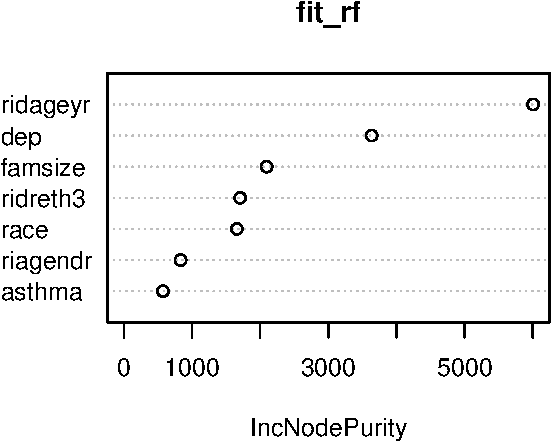
\includegraphics{07_OtherModels_files/figure-beamer/unnamed-chunk-21-1.pdf}

\end{frame}

\begin{frame}[fragile]{Random Forests}

We can see that age (\texttt{ridageyr}) is the most important variable,
depression (\texttt{dep}) follows, with the family size
(\texttt{famsize}) the third most important in the random forests model.

\end{frame}

\section{Conclusions}\label{conclusions}

\begin{frame}[fragile]{Conclusions}

Although we only discussed these methods briefly, that does not mean
they are less important. On the contrary, they are essential upper level
statistical methods. This brief introduction hopefully helped you know
what \texttt{R} is capable of across a wide range of methods.

\end{frame}
